\section{Sessions}
Une session est un regroupement de plusieurs groupes de processus. La participation d'un processus à une session est déterminée par son identifiant de session (SID). Le leader de session est le processus responsable de la création d'une nouvelle session et dont sont identifiant (PID) devient l'identifiant de session (SID) de cette session (généralement le shell). Lorsqu'un nouveau processus est créé, il hérite automatiquement de l'identifiant de session (SID) de son processus parent.

\subsection{Création d’une session}

\subsubsection{L’appel système \textit{setsid()} }

\begin{lstlisting}[frame=single]
#include <unistd.h>

pid_t setsid(void);
\end{lstlisting}

L’appel système \textit{setsid()} permet de créer une nouvelle session et définir le processus appelant comme le leader de cette session. Le PGID et SID deviennent le même que le PID du processus appelant.
Il est important de noter que, d'une part, un leader de groupe de processus existant ne peut pas créer une nouvelle session. D'autre part, lorsqu'un processus fait l'appel à \textit{setsid()}, il perd toute connexion préexistante au terminal de contrôle.

\subsection{Disposition des processus en groupes/sessions}

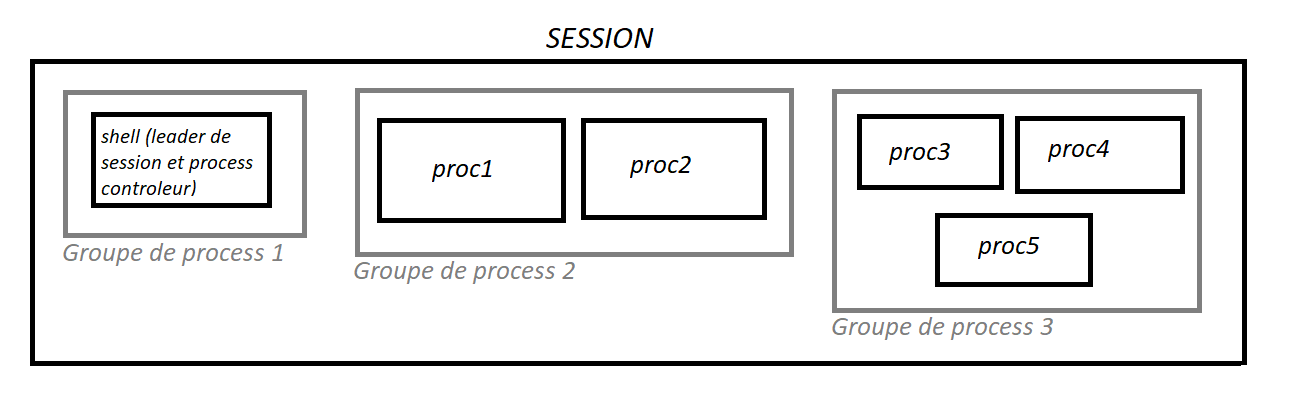
\includegraphics[width=1\textwidth]{img/SessionEtGroupes.png}